\renewcommand{\thesection}{\Roman{section}}
\titleformat{\section}
{\normalfont\bfseries}{PHẦN~\thesection.}{0.4em}{}
\titlespacing{\section}{0pt}{*0}{*0.5}
\begin{center}
	\begin{tabular}{M{10cm}M{8cm}}
		\textbf{TRƯỜNG THCS-THPT NGUYỄN KHUYẾN}& \textbf{ÔN TẬP KTTX LẦN 1 - HỌC KÌ 1}\\
		\textbf{MÃ ĐỀ: 001}& \textbf{Bài thi môn: VẬT LÝ 10}\\
		\textit{(Đề thi có 04 trang)}& \textit{Thời gian: 40 phút, không kể phát đề}
		
		\noindent\rule{4cm}{0.8pt} \\
	\end{tabular}
\end{center}
\vspace{-0.5cm}
\setcounter{section}{0}
		\section{Câu trắc nghiệm nhiều phương án lựa chọn}
		\textit{Thí sinh trả lời từ câu 1 đến câu 24. Mỗi câu hỏi thí sinh chọn một phương án}
		\setcounter{ex}{0}
		\Opensolutionfile{ans}[ans/G10C1TN]
		% ===================================================================
		\begin{ex}
			Đối tượng nghiên cứu của vật lí là gì?
			\choice
			{Các dạng vận động và tương tác của vật chất}
			{Quy luật tương tác của các dạng năng lượng}
			{\True Các dạng vận động của vật chất và năng lượng}
			{Quy luật vận động, phát triển của sự vật - hiện tượng}
			\loigiai{}
		\end{ex}
% ===================================================================
\begin{ex}
	Lĩnh vực nghiên cứu nào sau đây là của vật lí?	
	\choice
	{Nghiên cứu về sự thay đổi của các chất khi kết hợp với nhau}
	{Nghiên cứu sự phát triển của vi khuẩn}
	{Nghiên cứu về sự hình thành và phát triển của các tầng lớp, giai cấp trong xã hội}
	{\True Nghiên cứu về các dạng chuyển động và các dạng năng lượng khác nhau}
	\loigiai{}
\end{ex}
% ===================================================================
\begin{ex}
	Thành tựu nghiên cứu nào sau đây của Vật lí được coi là có vai trò quan trọng trong việc mở đầu cho cuộc cách mạng công nghệ lần thứ nhất?
	\choice
	{Nghiên cứu về lực vạn vật hấp dẫn}
	{\True Nghiên cứu về nhiệt động lực học}
	{Nghiên cứu về cảm ứng điện từ}
	{Nghiên cứu về thuyết tương đối}
	\loigiai{}
\end{ex}
% ===================================================================
\begin{ex}
	Trong các hoạt động dưới đây, hoạt động nào tuân thủ nguyên tắc an toàn khi sử dụng điện?
	\choice
	{Sửa chữa điện khi chưa ngắt nguồn điện}
	{Chạm tay trực tiếp vào ổ điện, dây điện trần hoặc dây dẫn điện bị hở}
	{Đến gần nhưng không tiếp xúc với các máy biến thế và lưới điện cao áp}
	{\True Kiểm tra mạch có điện bằng bút thử điện}
	\loigiai{}
\end{ex}
% ===================================================================
\begin{ex}
	Trong các hoạt động dưới đây, hoạt động nào tuân thủ nguyên tắc an toàn khi làm việc với các nguồn phóng xạ?
	\choice
	{Ăn uống, trang điểm trong phòng làm việc có chứa chất phóng xạ}
	{\True Sử dụng phương tiện phòng hộ cá nhân như quần áo phòng hộ, mũ, găng tay, áo chì, \dots}
	{Đổ rác thải phóng xạ tại các khu tập trung rác thải sinh hoạt}
	{Dùng hộp chứa bằng vật liệu thuỷ tinh để đựng chất phóng xạ}
	
	\loigiai{}
\end{ex}
% ===================================================================
\begin{ex}
	Công nghệ chất bán dẫn liên tục phá vỡ các rào cản để có thể tạo ra những con chip nhỏ hơn, nhanh hơn, mạnh hơn và tiết kiệm điện năng hơn. Vừa mới đây, IBM tuyên bố đã tạo ra một con chip $\SI{2}{\nano\meter}$.	Trong khi đó, kích thước trung bình của một gạo là $\SI{6}{\milli\meter}$. So với hạt gạo, con chip trên nhỏ hơn khoảng bao nhiêu lần?
	\begin{center}
		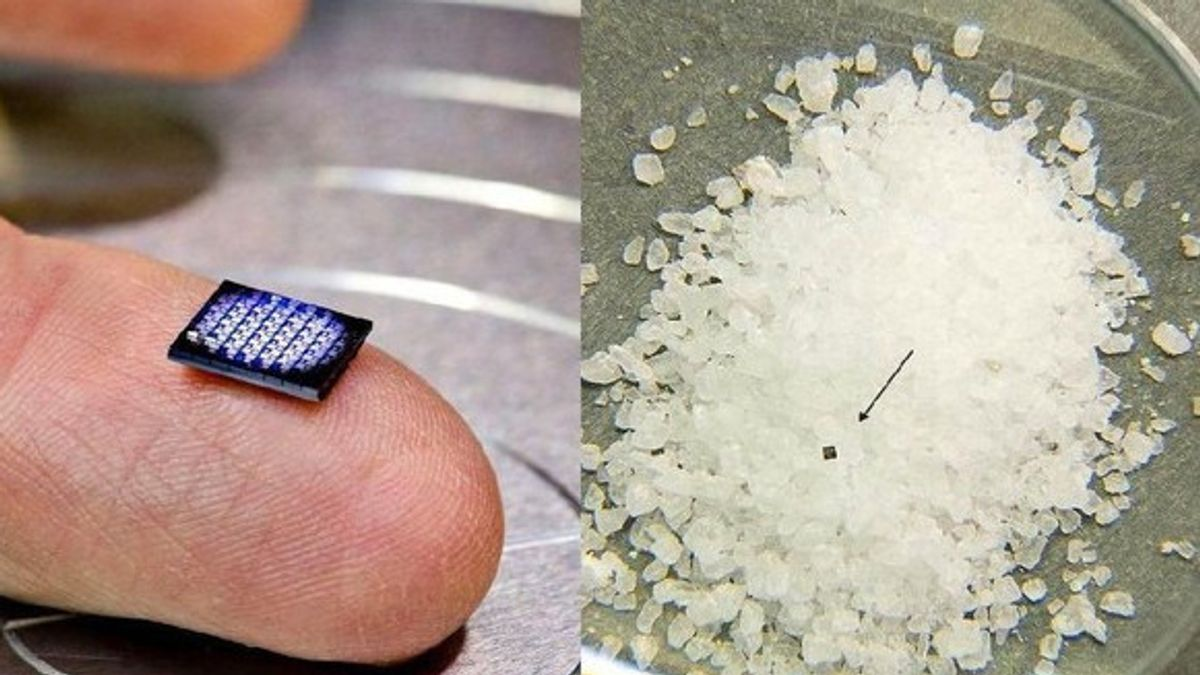
\includegraphics[width=0.4\linewidth]{figs/G10-CHUONG1-6}
		\captionof{figure}{So sánh kích thước chip $\SI{2}{\nano\meter}$ của IBM với các hạt gạo vỡ}
	\end{center}
	\choice
	{$3\cdot10^9$ lần}
	{\True $3\cdot10^6$ lần}
	{$3000$ lần}
	{$0,003$ lần}
	\loigiai{}
\end{ex}
% ===================================================================
\begin{ex}
	Chọn đáp án có từ /cụm từ thích hợp để hoàn thành bảng sau:
	\begin{center}
		\begin{tabular}{|c|c|c|}
			\hline
			\thead{Đơn vị} & \thead{Kí hiệu} & \thead{Đại lượng }\\
			\hline
			kelvin & (1) & (2)\\
			\hline
			ampe & $\si{\ampere}$ & (3)\\
			\hline
			candela & $\si{\candela}$ & (4)\\
			\hline
		\end{tabular}
	\end{center}
	\choice
	{(1) $\si{\kelvin}$; (2) Khối lượng; (3) Cường độ dòng điện; (4) Lượng chất}
	{\True (1) $\si{\kelvin}$; (2) Nhiệt độ; (3) Cường độ dòng điện; (4) Cường độ ánh sáng}
	{(1) $\si{\kelvin}$; (2) Nhiệt độ; (3) Cường độ dòng điện; (4) Lượng chất}
	{(1) $\si{\kelvin}$; (2) Khối lượng; (3) Cường độ dòng điện; (4) Cường độ ánh sáng}
	\loigiai{}
\end{ex}
% ===================================================================
\begin{ex}
	Đơn vị nào sau đây không thuộc thứ nguyên $L$ [Chiều dài]?
	\choice
	{Dặm}
	{Hải lí}
	{Năm ánh sáng}
	{\True Lạng}
	\loigiai{}
\end{ex}
% ===================================================================
\begin{ex}
	Chọn đáp án có từ/cụm từ thích hợp để hoàn thành các câu sau:
	\begin{itemize}
		\item[-] Các số hạng trong phép cộng (hoặc trừ) phải có cùng (1) \dots và nên chuyển về cùng (2) \dots.
		\item[-] (3) \dots của một biểu thức vật lí phải có cùng thứ nguyên.
	\end{itemize}
	\choice
	{(1) đơn vị; (2) thứ nguyên; (3)  Đại lượng}
	{(1) thứ nguyên; (2) đại lượng; (3) Hai vế}
	{(1) đơn vị; (2) đại lượng; (3) Hai vế}
	{\True (1) thứ nguyên; (2) đơn vị; (3) Hai vế}
	\loigiai{}
\end{ex}
% ===================================================================
\begin{ex}
	Trong các phép đo dưới đây, đâu là phép đo trực tiếp?
	\begin{enumerate}[label=(\arabic*)]
		\item Dùng thước đo chiều cao.
		\item Dùng cân đo cân nặng.
		\item Dùng cân và ca đong đo khối lượng riêng của nước.
		\item Dùng đồng hồ và cột cây số đo tốc độ của người lái xe.
	\end{enumerate}
	\choice
	{\True (1), (2)}
	{(1), (2), (4)}
	{(2), (3), (4)}
	{(2), (4)}
	\loigiai{}
\end{ex}
% ===================================================================
\begin{ex}
	Đáp án nào sau đây có 1 đơn vị cơ bản và 1 đơn vị dẫn xuất?
	\choice
	{mét, kilogram}
	{pascal, joule}
	{candela, kelvin}
	{\True newton, mol}
	\loigiai{}
\end{ex}


% ===================================================================
\begin{ex}
	Đại lượng đặc trưng cho tính chất nhanh hay chậm của chuyển động là 
	\choice
	{toạ độ}
	{gia tốc}
	{quãng đường đi}
	{\True tốc độ}
	\loigiai{}
\end{ex}
% ===================================================================
\begin{ex}
	Khi nhìn vào tốc kế của ô tô đang chạy, số chỉ trên tốc kế cho ta biết
	\choice
	{gia tốc tức thời của ô tô}
	{vận tốc tức thời của ô tô}
	{\True tốc độ tức thời của ô tô}
	{tốc độ trung bình của ô tô}
	\loigiai{}
\end{ex}
% ===================================================================
\begin{ex}
	Đâu là cách viết kết quả đo \textbf{đúng}?
	\choice
	{$A=\overline{A}+\Delta A$}
	{$A=\overline{A}-\Delta A$}
	{\True $A=\overline{A}\pm\Delta A$}
	{$A=\overline{A}:\Delta A$}
	\loigiai{}
\end{ex}

% ===================================================================
\begin{ex}
	Giá trị nào sau đây có 2 chữ số có nghĩa (CSCN)?
	\choice
	{\True $\SI{210}{\meter}$}
	{$\SI{20}{\meter}$}
	{$\SI{0.02}{\meter}$}
	{$\SI{201}{\meter}$}
	\loigiai{}
\end{ex}
% ===================================================================
\begin{ex}
	Sai số tương đối của đại lượng $A$ được tính bởi công thức	
	\choice
	{\True $\delta A=\dfrac{\Delta A}{\overline{A}}\cdot\SI{100}{\percent}$}
	{$\overline{\Delta A}=\dfrac{\Delta A_1+\Delta A_2+\dots+\Delta A_n}{n}$}
	{$A=\overline{A}\pm\Delta A$}
	{$\delta A=\dfrac{\overline{A}}{\Delta A}$}
	\loigiai{}
\end{ex}

% ===================================================================
\begin{ex}
	Một học sinh dùng thước đo chiều dài của chiếc bút chì như hình bên dưới. Nếu lấy sai số dụng cụ bằng 1 nửa độ chia nhỏ nhất thì sai số hệ thống trong phép đo trên là	
	\begin{center}
		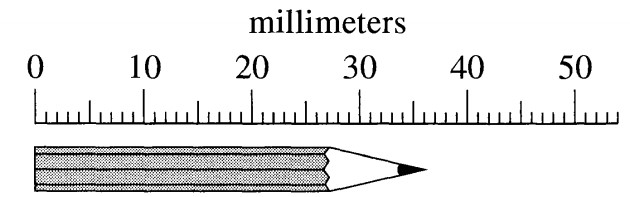
\includegraphics[width=0.4\linewidth]{figs/G10-CHUONG1-1}
	\end{center}
	\choice
	{$\SI{1}{\milli\meter}$}
	{\True $\SI{0.5}{\milli\meter}$}
	{$\SI{1}{\centi\meter}$}
	{$\SI{0.5}{\milli\meter}$}
	\loigiai{}
\end{ex}

% ===================================================================
\begin{ex}
	Một bánh xe có bán kính $R=\xsi{10\pm0,5}{\centi\meter}$. Sai số tương đối của chu vi bánh xe là
	\choice
	{$\SI{0.05}{\percent}$}
	{\True $\SI{5}{\percent}$}
	{$\SI{10}{\percent}$}
	{$\SI{25}{\percent}$}
	\loigiai{
		$$\delta R=\dfrac{\Delta R}{\overline{R}}\cdot\SI{100}{\percent}=\SI{5}{\percent}.$$	
	}
\end{ex}
% ===================================================================
\begin{ex}
	Thứ nguyên của vận tốc là
	\choice
	{$LT$}
	{$L^{-1}T$}
	{$L^{-1}T^{-1}$}
	{\True $LT^{-1}$}
	\loigiai{
		\begin{eqnarray*}
			v&=&\dfrac{s}{t}\\
			\Rightarrow \left[v\right]&=&\dfrac{\left[s\right]}{\left[t\right]}=LT^{-1}.
		\end{eqnarray*}	
	}
\end{ex}
% ===================================================================
\begin{ex}
	Cho thứ nguyên của trọng lượng là $MLT^{-2}$. Thứ nguyên của trọng lượng riêng là
	\choice
	{$MLT^{-1}$}
	{$MLT^{-2}$}
	{$ML^{-2}T^{-1}$}
	{\True $ML^{-2}T^{-2}$}
	\loigiai{
		\begin{eqnarray*}
			d&=&\dfrac{P}{V}\\
			\Rightarrow \left[d\right]&=&\dfrac{\left[P\right]}{\left[V\right]}\\
			\Leftrightarrow \left[d\right]&=&\dfrac{MLT^{-2}}{L^3}=ML^{-2}T^{-2}.
		\end{eqnarray*}	
	}
\end{ex}
% ===================================================================
\begin{ex}
	Một xe xuất phát từ lúc 7 giờ 15 phút sáng từ thành phố M, chuyển động thẳng đều tới thành phố N, cách thành phố M $\SI{90}{\kilo\meter}$. Biết tốc độ của xe là $\SI{60}{\kilo\meter/\hour}$, xe đến thành phố N lúc	
	\choice
	{9 giờ 45 phút}
	{8 giờ 30 phút}
	{9 giờ 30 phút}
	{\True 8 giờ 45 phút}
	\loigiai{
		Thời gian để xe đi từ M đến N:
		$$\Delta t=\dfrac{s}{v}=\SI{1.5}{\hour}.$$
		Thời điểm xe đến N:
		$$t=\SI{7}{\hour}\SI{15}{\minute}+\Delta t=\SI{8}{\hour}\SI{45}{\minute}.$$	
	}
\end{ex}
% ===================================================================
\begin{ex}
	Một vận động viên chạy cự li $\SI{600}{\meter}$ mất $\SI{74.75}{\second}$. Tốc độ trung bình của vận động viên đó là
	\choice
	{\True $\SI{8.03}{\meter/\second}$}
	{$\SI{9.03}{\meter/\second}$}
	{$\SI{10.03}{\meter/\second}$}
	{$\SI{11.03}{\meter/\second}$}
	\loigiai{
		Tốc độ trung bình của vận động viên:
		$$v_\text{tb}=\dfrac{s}{\Delta t}=\SI{8.03}{\meter/\second}.$$	
	}
\end{ex}
% ===================================================================
\begin{ex}
	Một người bơi dọc theo chiều dài $\SI{55}{\meter}$ của bể bơi hết $\SI{50}{\second}$ rồi quay về lại chỗ xuất phát trong $\SI{60}{\second}$. Trong suốt quãng đường đi và về vận tốc trung bình của người đó là
	\choice
	{\True $\SI{0}{\meter/\second}$}
	{$\SI{1.0}{\meter/\second}$}
	{$\SI{1.1}{\meter/\second}$}
	{$\SI{2.0}{\meter/\second}$}
	\loigiai{
		Vì điểm đầu của quĩ đạo chuyển động trùng với điểm cuối nên $d=0\Rightarrow v=0$.	
	}
\end{ex}

% ===================================================================
\begin{ex}
	Hình bên là đồ thị toạ độ - thời gian của một chiếc xe máy đang chạy trên đường thẳng. Xe này có tốc độ là
	\begin{center}
		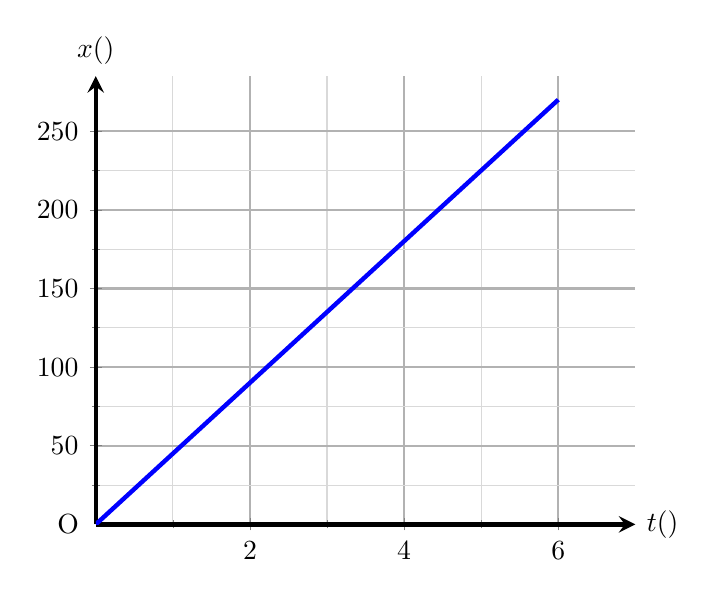
\begin{tikzpicture}  
			\begin{axis}[  ultra thick,
				xmin=0,  
				xmax=7,  
				xtick={0,2,...,6},
				ytick={0,50,...,250},
				minor x tick num=1,
				minor y tick num=1,
				ymin=0,  
				ymax=285, 
				samples=300,
				axis lines=center, 
				grid style={step=1, line width =0.4pt, color=gray!30!white},
				grid=both, %giới hạn ô lưới
				major grid style={line width=0.8pt,gray!60!white},
				xlabel=$\xsi{t}{\left(\si{\hour}\right)}$, 		ylabel=$\xsi{x}{\left(\si{\kilo\meter}\right)}$,
				every axis y label/.style={at=(current axis.above origin),anchor=south},  
				every axis x label/.style={at=(current axis.right of origin),anchor=west},  ] 
				\addplot [ultra thick, blue, smooth, domain=0:6] {45*x}; 
			\end{axis} 
			\node at (-0.35,0) {O}; 
		\end{tikzpicture}
		
	\end{center}
	\choice
	{\True $\SI{45}{\kilo\meter/\hour}$}
	{$\SI{43.75}{\kilo\meter/\hour}$}
	{$\SI{45.45}{\kilo\meter/\hour}$}
	{$\SI{50}{\kilo\meter/\hour}$}
	\loigiai{
		Tại $t=\SI{5}{\hour}$ thì $x=\SI{225}{\kilo\meter}$:
		$$\left|v\right|=\left|\dfrac{\Delta x}{\Delta t}\right|=\SI{45}{\kilo\meter/\hour}.$$	
	}
\end{ex}


\Closesolutionfile{ans}
\section{Câu trắc nghiệm đúng/sai} 
\textit{Trong mỗi ý \textbf{a)}, \textbf{b)}, \textbf{c)}, \textbf{d)} ở câu bên dưới, thí sinh chọn đúng hoặc sai}
\setcounter{ex}{0}
\Opensolutionfile{ans}[ans/G10C1TF]
% ===================================================================
\begin{ex}
	Một bạn học sinh dùng volt kế để đo hiệu điện thế hai đầu điện trở. Kết quả trong một lần đo được ghi nhận như hình bên dưới.
	\begin{center}
		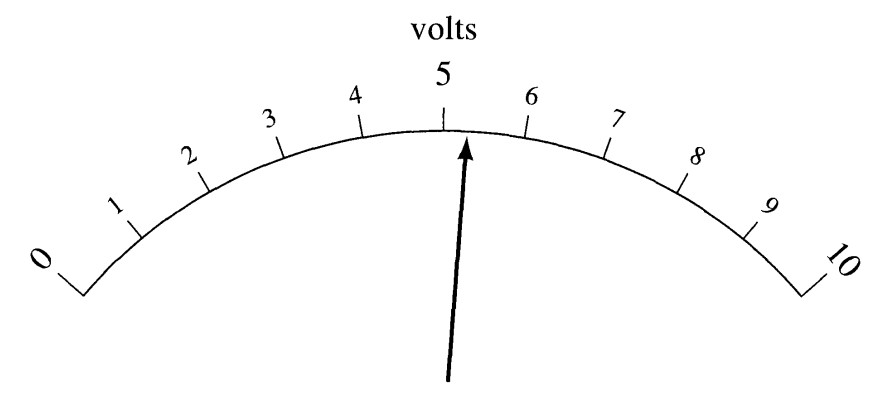
\includegraphics[width=0.6\linewidth]{figs/G10-CHUONG1-2}
	\end{center}
	\choiceTF[t]
	{\True Độ chia nhỏ nhất của volt kế trên là $\SI{1}{\volt}$}
	{Kết quả lần đo trên hình nên được đọc là $\SI{5.25}{\volt}$}
	{Có thể hạn chế sai số hệ thống bằng cách thực hiện phép đo nhiều lần}
	{\True Kết quả đo có thể mắc sai số ngẫu nhiên do thao tác của người đo hoặc các yếu tố bên ngoài tác động}
	\loigiai{
		\begin{itemchoice}
			\itemch Đúng.
			\itemch Sai. ĐCNN của volt kế là $\SI{1}{\volt}$ nên chỉ có thể đọc được giá trị $\SI{5}{\volt}$ hoặc $\SI{6}{\volt}$. Quan sát chủ quan thấy kim nằm gần vạch $\SI{5}{\volt}$ hơn.
			\itemch Sai. Sai số hệ thống được hạn chế bằng cách dùng dụng cụ có độ chia nhỏ nhất càng nhỏ và hiệu chỉnh dụng cụ đo về 0 trước khi đo.
			\itemch Đúng.
		\end{itemchoice}	
		
	}
\end{ex}

\Closesolutionfile{ans}
\section{Câu trắc nghiệm trả lời ngắn} \textit{Thí sinh trả lời từ câu 1 đến câu 6}
\setcounter{ex}{0}
\Opensolutionfile{ans}[ans/G10C1TL]
% ===============================================================
\begin{ex}
	Hố đen là một trong những đối tượng rất đặc biệt trong vũ trụ. Nguồn gốc ra đời của hố đen bắt nguồn từ sự suy sụp hấp dẫn của một vật thể khối lượng rất lớn vào một điểm kỳ dị và tạo ra quanh nó một vùng không - thời gian cong vô hạn, nơi mà không thứ gì có thể thoát ra từ đó, kể cả ánh sáng. 
	\begin{center}
		\begin{tabular}{M{7.5cm}M{7.5cm}}
			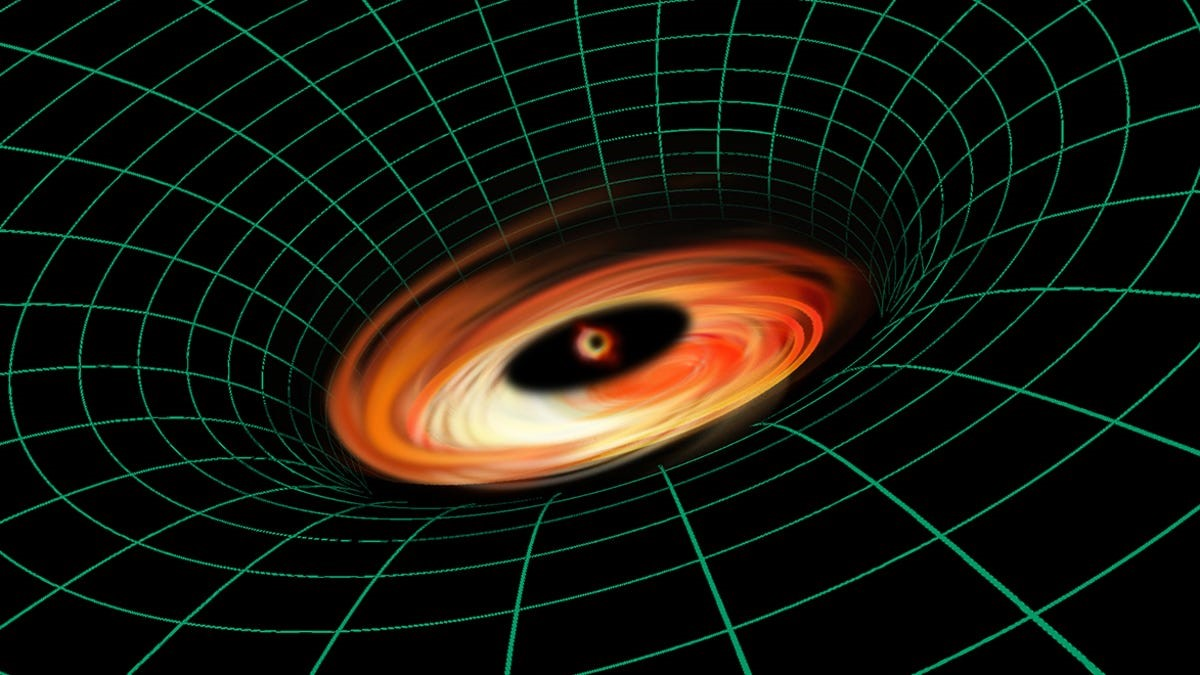
\includegraphics[width=0.7\linewidth]{figs/G10-CHUONG1-4}
			&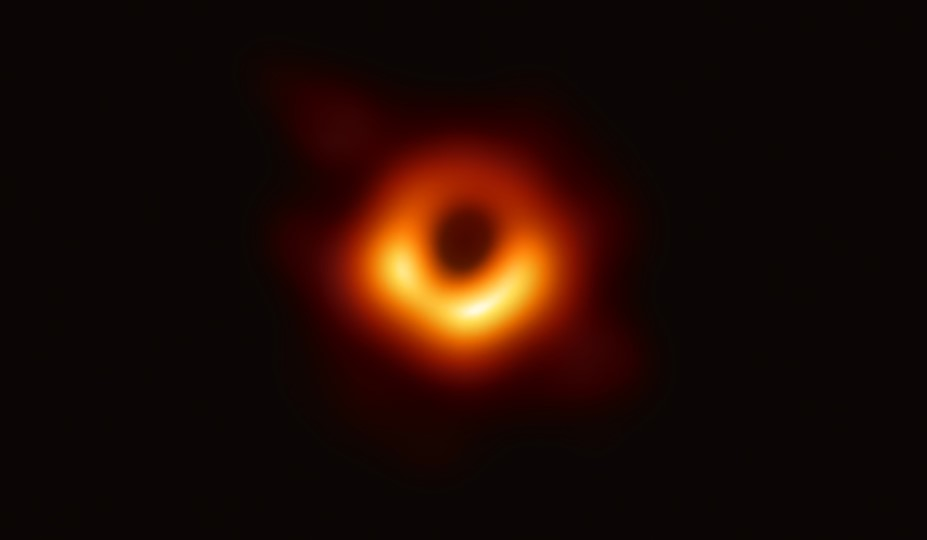
\includegraphics[width=0.7\linewidth]{figs/G10-CHUONG1-5}\\
			\textit{Minh hoạ hố đen làm cong không - thời gian}& \textit{Ảnh hố đen chụp bởi Kính viễn vọng chân trời sự kiện (EHT) và công bố năm 2019} 
		\end{tabular}
	\end{center}
	Theo nhà vật lí học người Đức Karl Schwarzschild, một vật thể có kích thước bằng với bán kính giới hạn (bán kính Schwarzschild) thì nó sẽ trở thành một hố đen. Bán kính  Schwarzschild được cho bởi công thức:
	$$R_S=\dfrac{2GM}{c^2}$$
	Trong đó:
	\begin{itemize}
		\item $R_S$ là bán kính hấp dẫn Schwarzschild;
		\item $G$ là hằng số hấp dẫn;
		\item $M$ là khối lượng vật thể;
		\item $c$ là tốc độ ánh sáng trong chân không.
	\end{itemize}
	Trong công thức trên, hằng số hấp dẫn có thứ nguyên là $L^\alpha M^{-\beta}T^{-\gamma}$. Với $\alpha$, $\beta$, $\gamma$ là các số nguyên dương. Xác định giá trị của $\alpha\beta\gamma$.
	
	\shortans{312 }
	\loigiai{
		Ta có:
		$$G=\dfrac{1}{2}\dfrac{R_Sc^2}{M}.$$
		Phân tích thứ nguyên:
		$$\left[G\right]=\dfrac{\left[R_S\right]\times\left[c\right]^2}{\left[M\right]}=\dfrac{L\times\left(LT^{-1}\right)^2}{M}=L^3M^{-1}T^{-2}\Rightarrow \begin{cases}
			\alpha=3\\
			\beta=1\\
			\gamma=2
		\end{cases}.$$
	}
\end{ex}
% ===============================================================
\begin{ex}
	Một nhóm học sinh đo được hiệu điện thế giữa hai đầu một điện trở là $U=\xsi{\left(10,0\pm0,3\right)}{\volt}$ và cường độ dòng điện qua điện trở là $I=\xsi{\left(1,3\pm0,2\right)}{\ampere}$. Tính sai số tương đối trong phép đo điện trở \textit{(Kết quả tính theo đơn vị $\si{\percent}$ và làm tròn đến 3 CSCN)}.\\
	Cho biết giá trị của điện trở được xác định bởi $R=\dfrac{U}{I}$.
	\shortans{18,4 }
	\loigiai{
		Giá trị điện trở:
		$$R=\dfrac{U}{I}.$$
		Sai số tương đối của phép đo:
		$$\delta R=\left(\dfrac{\Delta U}{\overline{U}}+\dfrac{\Delta I}{\overline{I}}\right)\cdot\SI{100}{\percent}\approx\SI{18.4}{\percent}.$$
	}
\end{ex}
\textit{Dữ kiện sau đây được dùng chung cho câu 3 đến câu 6}\\
Bạn An thực hiện thí nghiệm đo tốc độ chuyển động thẳng với dụng cụ và sơ đồ bố trí thí nghiệm như hình bên dưới.
Trong đó, hai cổng quang điện A và B được đặt cách nhau $\SI{30}{\centi\meter}$ và được nối với đồng hồ đo thời gian hiện số (1) được đặt ở chế độ đo với sai số dụng cụ $\SI{0.01}{\second}$. Độ chia nhỏ nhất của thước đo (5) là $\SI{0.5}{\centi\meter}$.
\begin{center}
	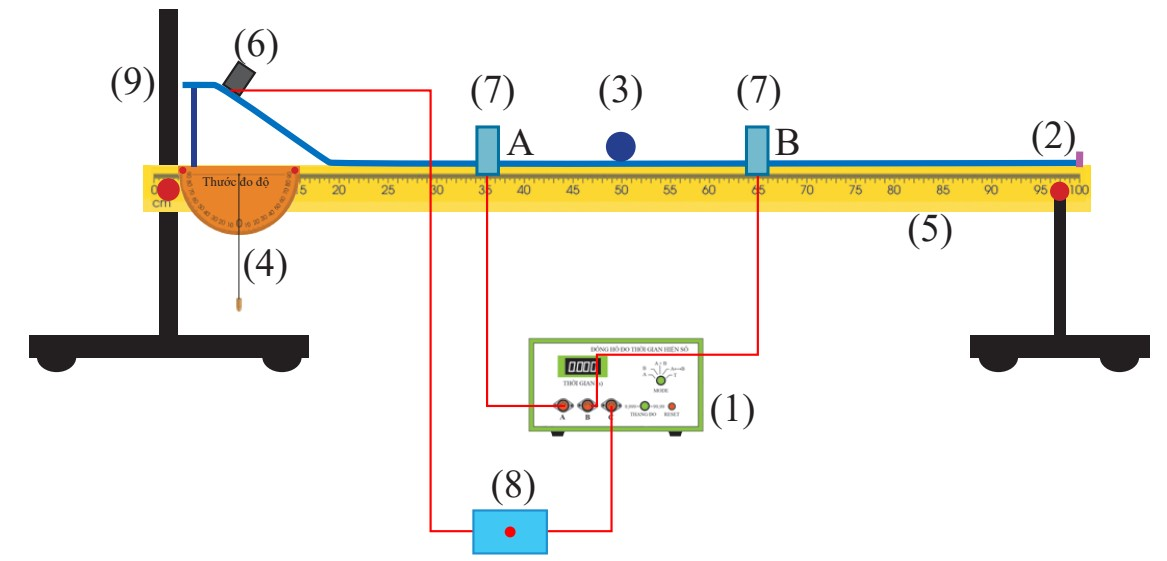
\includegraphics[width=0.75\linewidth]{figs/G10-CHUONG1-3}
\end{center}
Bạn An thiết đặt đồng hồ đo thời gian hiện số ở chế độ A$\leftrightarrow$B để đo thời gian viên bi chuyển động kể từ khi chắn qua cổng quang A đến khi qua cổng quang B. Sau 5 lần đo, An ghi nhận được các giá trị thời gian chuyển động của viên bi như bảng bên dưới:
\begin{center}
	\begin{longtable}{|M{4cm}|M{2cm}|M{2cm}|M{2cm}|M{2cm}|M{2cm}|}
		\hline
		\thead{Lần đo}&1&2&3&4&5\\
		\hline
		\thead{Thời gian $\left(\si{\second}\right)$}& 4,75 & 4,68 & 4,73 & 4,68 & 4,70\\
		\hline
	\end{longtable}
\end{center}
\textit{* Lưu ý: Trong các phần tính toán bên dưới, các giá trị trung bình được lấy cùng bậc thập phân với giá trị đo.}
% ===============================================================
\begin{ex}
	Xác định thời gian chuyển động trung bình của viên bi \textit{(Kết quả tính theo đơn vị giây và làm tròn đến 3 CSCN)}.
	\shortans{4,71}
	\loigiai{
		Thời gian chuyển động trung bình của viên bi:
		$$\overline{t}=\dfrac{t_1+t_2+\dots+t_5}{5}=\SI{4.708}{\second}\approx\SI{4.71}{\second}.$$	
	}
\end{ex}
% ===============================================================
\begin{ex}
	Xác định sai số tương đối trong phép đo thời gian trên \textit{(Kết quả tính theo đơn vị $\si{\percent}$ và làm tròn đến 2 CSCN)}.
	\shortans{0,85}
	\loigiai{
		\begin{center}
			\begin{longtable}{|M{2cm}|M{4cm}|M{2cm}|}
				\hline
				\thead{Lần đo} & $\xsi{t}{\left(\second\right)}$ &$\xsi{\Delta t}{\left(\second\right)}$\\
				\hline
				1 & 4,75 &0,04 \\
				\hline
				2 & 4,68 & 0,03\\
				\hline
				3 & 4,73 & 0,02\\
				\hline
				4 & 4,68 & 0,03\\
				\hline
				5 & 4,70 & 0,01\\
				\hline
				\thead{TB}&4,71&0,03\\
				\hline
			\end{longtable}
		\end{center}
		Sai số tuyệt đối của phép đo thời gian:
		$$\Delta t=\overline{\Delta t}+\Delta t_{\text{dc}}=\SI{0.03}{\second}+\SI{0.01}{\second}=\SI{0.04}{\second}.$$
		Sai số tương đối của phép đo thời gian:
		$$\delta t=\dfrac{\Delta t}{\overline{t}}\cdot\SI{100}{\percent}=\dfrac{\SI{0.04}{\second}}{\SI{4.71}{\second}}\cdot\SI{100}{\percent}\approx\SI{0.85}{\percent}.$$}
\end{ex}
% ===============================================================
\begin{ex}
	Xác định tốc độ trung bình của viên bi trong thí nghiệm trên \textit{(Kết quả tính theo đơn vị $\si{\centi\meter/\second}$ và làm tròn đến 2 CSCN)}.
	\shortans{6,37}
	\loigiai{
		$$\overline{v}=\dfrac{\overline{s}}{\overline{t}}=\dfrac{\SI{30}{\centi\meter}}{\SI{4.71}{\second}}\approx\SI{6.37}{\centi\meter/\second}.$$
	}
\end{ex}
% ===============================================================
\begin{ex}
	Xác định sai số tuyệt đối trong phép đo tốc độ trung bình của viên bi \textit{(Kết quả tính theo đơn vị $\si{\centi\meter/\second}$ và làm tròn đến 2 CSCN)}.
	\shortans{0,11}
	\loigiai{
		ĐCNN của thước (5) là $\SI{0.5}{\centi\meter}$ nên sai số $\Delta s=\dfrac{\SI{0.5}{\centi\meter}}{2}=\SI{0.25}{\centi\meter}$.\\
		Sai số tuyệt đối trong phép đo tốc độ trung bình:
		$$\dfrac{\Delta v}{\overline{v}}=\dfrac{\Delta s}{\overline{s}}+\dfrac{\Delta t}{\overline{t}}\Rightarrow \Delta v=\left(\dfrac{\Delta s}{\overline{s}}+\dfrac{\Delta t}{\overline{t}}\right)\cdot\overline{v}=\left(\dfrac{\SI{0.25}{\centi\meter}}{\SI{30}{\centi\meter}}+\dfrac{\SI{0.04}{\second}}{\SI{4.71}{\second}}\right)\cdot\left(\SI{6.37}{\centi\meter/\second}\right)\approx\SI{0.11}{\centi\meter}.$$
	}
\end{ex}
\Closesolutionfile{ans}
\begin{center}
	\textbf{--- HẾT ---}
\end{center}
\newpage
\setcounter{section}{0}
\begin{center}
	\textbf{\large BẢNG ĐÁP ÁN}
\end{center}
\section{}
\inputansbox{10}{ans/G10C1TN}
\section{}
\inputansbox[2]{2}{ans/G10C1TF}
\section{}
\inputansbox[3]{6}{ans/G10C1TL}